\documentclass{standalone}

\usepackage{graphicx}
\usepackage{tikz}
\usepackage{standalone}
\usepackage{amsmath}
\usepackage{amssymb}
\usepackage{makecell}
\usetikzlibrary{positioning}
\usetikzlibrary{shapes.geometric}

\begin{document}
%\begin{standalone}

\begin{tikzpicture}

\node[anchor=south west, inner sep=0] (image) at (0,0) {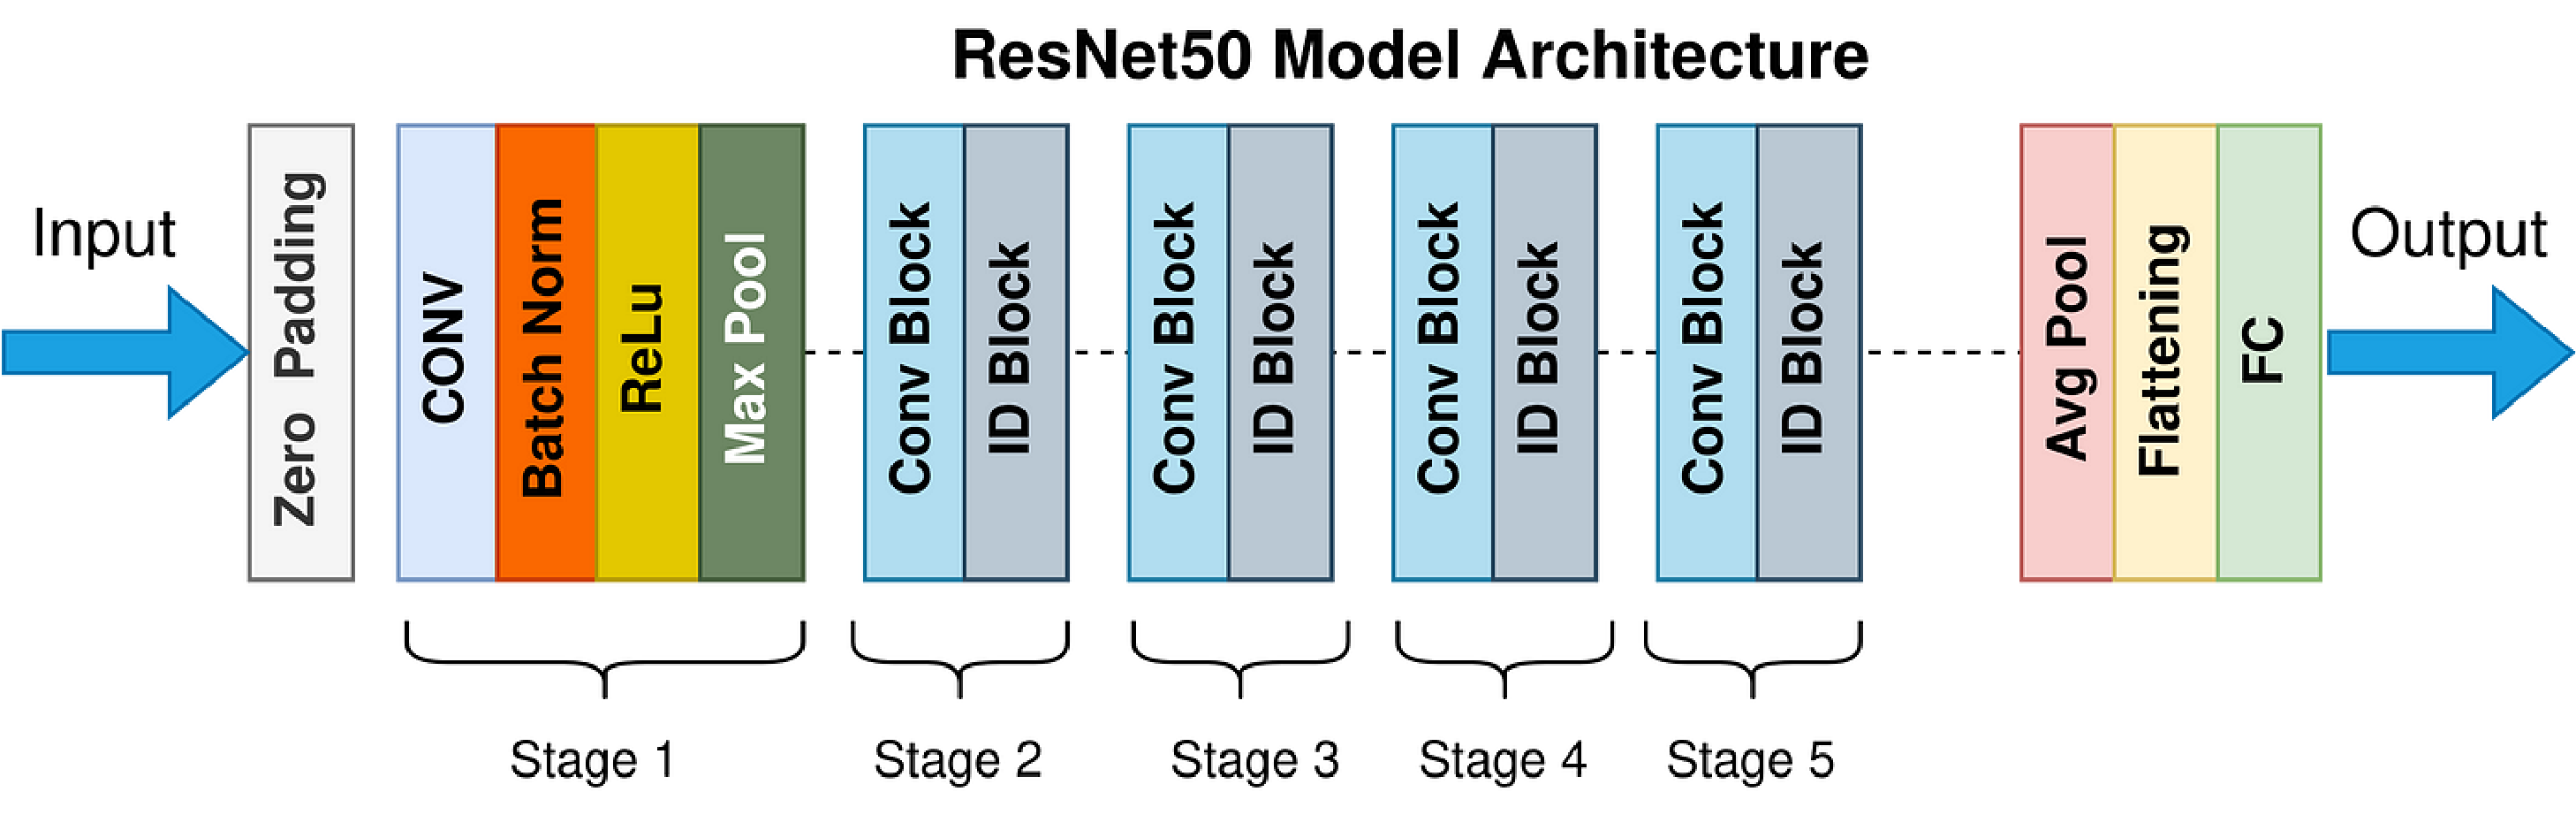
\includegraphics[width=0.45\linewidth]{structure.pdf}};
\node[right=0.5cm of image, font=\large, xshift=0.05\linewidth] (text) { covariance $\sum_tg_tg_t^\top\in\mathbb{R}^{d\times d}$ };
\node[below=0.5cm of image, font=\large] {\makecell[c]{Parameters $x_t\in\mathbb{R}^d$ \\ with $d\approx 23\times 10^6$.}};
\node[regular polygon,regular polygon sides=4, draw, line width=2pt, anchor=north, below=0.1cm of text, inner sep=-1em]  {$\ \ \quad>2\mathrm{PB}\quad\ \ $};
\end{tikzpicture}

%\end{standalone}
\end{document}
